\documentclass{article}
\usepackage{amssymb}
\usepackage{amsmath}
\usepackage{setspace}
\usepackage{graphicx}
\usepackage{algorithm}
\usepackage{algorithmicx}
\usepackage[noend]{algpseudocode}
\usepackage{hyperref}
\usepackage{graphicx}
\hypersetup{
    colorlinks=true,
    linkcolor=blue,
    filecolor=magenta,      
    urlcolor=cyan,
    }
%\usepackage[margin=1in]{geometry}
\title{CS395 Spring 2018---Final Project Report \\ \large Heart Rate Prediction with Deep Video Regression}
\author{
  Adam Barson \\ \small{\texttt{abarson@uvm.edu}}
  \and Daniel Berenberg \\ \small{\texttt{djberenb@uvm.edu}
  \thanks{in collaboration with Dr. Ryan McGinnis, UVM} 
 \thanks{under advisory of Dr. Safwan Wsah, UVM}}
}
\date{\today}
\onehalfspace
\begin{document}
\maketitle
\section[1]{Introduction}
\noindent Millions of Americans are afflicted with panic disorder [1], a psychiatric disorder in which debilitating fear and anxiety arise with no apparent cause [2]. There are several clinically available methods to treat panic disorder, many of which involve either medication or intensive psychotherapy [3]. Past research [4] in the biomedical field has shown that by simply showing a panic disorder victim their heart rate on the onset of or during a panic attack, their episode was significantly mitigated or weakened in intensity.

\noindent Allowing people afflicted with panic disorder to access vitals such as heart rate and respiratory rate could not only benefit the longer term management of the disorder, but mitigate the risks and side effects of a live panic attack.

\noindent In order to expose this treatment method to as many victims of panic disorder as possible, we explore an element of the solution by making use of the ubiquitous smartphone. There is promising evidence that suggests pulse is detectable by processing videos in smartphone cameras. By pressing a finger against a smartphone camera with the flashlight activated, we can obtain a highly resolved clip of the blood pulsating within the finger. This project aims to leverage deep learning techniques in order to predict a patient?s heart rate from such a video. 
\section[2]{Problem Definition}
%%%%%%%%%%%%%%%%%%%%%%%%%%%%%%%%%%%%%%%%%%%%
\subsection[2.1]{Task Definition}
\noindent Our objective is to produce a fast, accurate within a small squared error, model that, given a sequence of the above described frames $S$ of images $X_{i} \ldots X_{n}$, we output a value $h{r}$, the heart rate of the individual who submitted the sequence. 

\noindent This problem is specifically intriguing not only for its real world application but because the task is vastly more dependent on the the temporal axis than other neural video processing tasks. 

\noindent The dataset used by this project has been provided by Dr. Ryan McGinnis of the University of Vermont Biomedical Engineering department. Video data was collected by sampling $31$ separate subjects; each patient recorded two videos of their finger-- one at a resting heart rate, and one after an intense $60$ second workout. All of the raw videos gathered during the study are around 30 seconds long. For each sample $V$, the heart rate $h_{r}$ and respiratory rate $r{v}$ for each were also recorded and are provided along with the video data.

\subsection[2.2]{Algorithm Definitions and Related Work}
\noindent There are various algorithms that apply to deep neural video processing tasks; we explored three: 2D stacked convolutions with a subsequent LSTM layer or LRCN [5], Two stream networks that incorporate the use of optical flow [6], and 3D-Convolution [7]. Each of these models is designed to extract features from the temporal element of the sample in a unique way.

\noindent The \textbf{LRCN} uses stacked convolutional layers in order to extract hierarchical, semantically meaningful feature vectors which are then fed into an LSTM layer which uses these features to determine long term dependencies throughout the sample. 

\noindent A \textbf{two stream network} uses two forms of input: raw frame sequences and the corresponding sequence of optical flow images that describes the change between some pair of frames. Formally, optical flow is defined as the pattern of apparent motion of objects, surfaces, and edges in a visual scene caused by the relative motion between an observer and the scene [8]. Since the optical flow transformation embeds temporal data in a 2D image, the two stream CNN is entirely a convolutional neural network with some sequence of dense layers at the end. Our adaptation of the two stream CNN adopts the temporal stream of the data and leaves the spatial stream. As noted previously, each frame is inconsequential in determining the heart rate of the video; the temporal correlations and color variations over time are much more semantically meaningful.

Finally, our third perspective on video regression stems from the 3D convolutional network, which considers a volume and convolves throughout it, learning hierarchical features and passing it to the next layer. Initially, each of these models was a network which had a single, linearly activated output node for regression. Ultimately, we also experimented with scaling the data to fall within the range of -1 to 1, which our LSTM models benefitted from. Out of all the models that were each tested, the 3D CNN ultimately performed the best.

Initially, each of these models was a network which had a single, linearly activated output node for regression. Ultimately, we also experimented with scaling the data to fall within the range of -1 to 1, which our LSTM models benefitted from. Out of all the models that were each tested, the 3D CNN ultimately performed the best.

%%%%%%%%%%%%%%%%%%%%%%%%%%%%%%%%%%%%%%%%%%%%
\section[3]{Experimental Evaluation}
\subsection[3.1] {Methodology}
\noindent Since our output is a single, real valued number, we use the mean squared error (MSE) and root mean squared error (RMSE) metrics in order to summarize the performance of the model at a given point.

\noindent Since our dataset consisted of about 16 videos altogether, we used various on-the-fly (runtime) and offline (hard disk) augmentation techniques. Our runtime techniques consisted mainly of random perturbations to images in the way of aphine transformations such as rotation, shear. Through several iterations, we eventually settled on scaling the speed of all videos in our dataset by all decade factors $a \in [0.5, 2.0]$ and assigning each of those newly augmented videos a label of $h_{r}a$, where $h_{r}$ is the heart rate of the original video. 

Below shows the dataset distribution before and after the augmentation steps. The left shows that the original distribution was sparsely, unevenly distributed and the resulting augmented set seems to simulate a more densely a uniformly distributed dataset.
\begin{center}
\begin{figure}[htb]
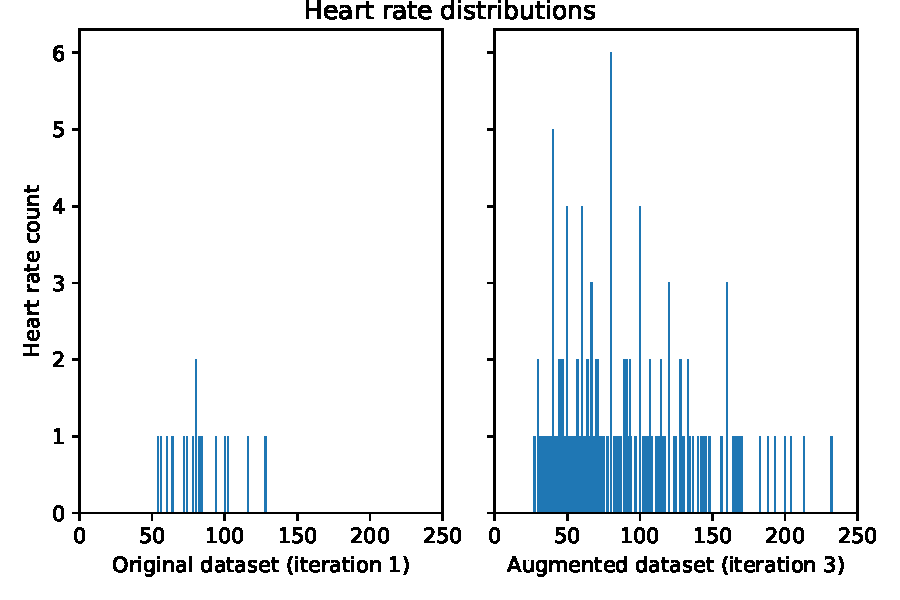
\includegraphics[width=0.7\textwidth]{figs/dataset_distrib.pdf}
\label{fig:distrib}
\caption{Dataset distribution before and after augmentation.}
\end{figure}
\end{center}
%%%%%%%%%%%%%%%%%%%%%%%%%%%%%%%%%%%%%%%%%%%%
\subsection[3.2] {Experiments}
%%%%%%%%%%%%%%%%%%%%%%%%%%%%%%%%%%%%%%%%%%%%
\subsubsection[3.2.1]{Preliminary Investigation}
In order to assess the feasibility of this task, we aimed to build a simple classifier to differentiate between low and high heart rates. We explored two models of the three: the Long-term Recurrent CNN (LRCN), and a variant of a 3D CNN.
Our results proved to be fairly promising. The LRCN yielded a 90\% classification accuracy, while the 3D CNN yielded around 70\%.

%%%%%%%%%%%%%%%%%%%%%%%%%%%%%%%%%%%%%%%%%%%%
\subsubsection[3.2.2]{Intermediary Experiments}
Given the initial success of the LRCN in classifying low and high heart rates, we naturally were interested in extending its capabilities for regression. To do so, we simply replaced the 2 node softmax activation dense layer with a 1 node linear activation dense layer. We tested several variants of LRCN models repurposed for regression-- namely, a LRCN with two extra dense layers before the output neuron, and a LRCN that employed a stacked LSTM.

Given the power of 3D CNNs in exploiting the temporal nature of videos, we also explored various 3D CNN architectures. These included the C3D network [9], and a slightly stripped down variant. The C3D model, while powerful, proved to be incredibly cumbersome to run. 50 epochs-- around 20,000 iterations through the data-- took 50 hours to complete.
\begin{center}
\begin{figure}[htb]
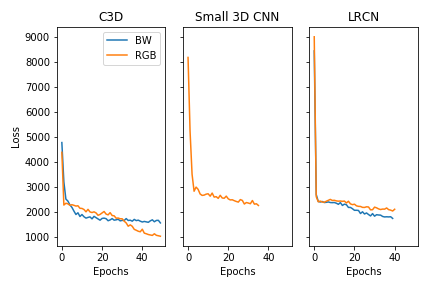
\includegraphics[width=0.8\textwidth]{figs/losses.png}
\label{fig:distrib}
\caption{Dataset distribution before and after augmentation.}
\end{figure}
\end{center}

In retrospect, it may not be a wise choice to use LSTMs for this type of task, given that the LSTM seeks to discover long term dependencies, which are at best very weak in a regular motion such as the beating of a pulse. Hence, we were directed towards the 3D CNN, despite its computational load. The threat of computational load caused us to experiment with CNNs and LSTMs further to no avail, the results of which are omitted due to irrelevance.
%%%%%%%%%%%%%%%%%%%%%%%%%%%%%%%%%%%%%%%%%%%%
\subsubsection[3.2.3]{Temporal Stream}
We decided to investigate optical flow by computing adjacent optical flow (the motion relative displacement between two adjacent frames) using python's \texttt{cv2} library. The rationale behind this choice was the fact that optical flow data not only embeds the temporality in the spatial, frame level context, but also because the shear pixel variation applied 
%%%%%%%%%%%%%%%%%%%%%%%%%%%%%%%%%%%%%%%%%%%%
\subsubsection[3.2.4]{3D CNN Experiments}
In the $11^{th}$ hour of the project?s deadline, we revisited the 3D CNN, addressing the previous challenge of its computational demand by decreasing the size of our sequence frames to 32x32x1 and decreasing the size of our original network. This reduction in size brought increased our processing time by at least 100 fold, meaning the 3D CNN was suddenly viable for training. This iteration of experimental models were meant to determine whether or not the 3D CNN was viable. The results are forthcoming and will be provided in a subsequent release regarding this work, but they look quite promising, reaching best-yet MSE.
%%%%%%%%%%%%%%%%%%%%%%%%%%%%%%%%%%%%%%%%%%%%
\subsection[3.3] {Discussion}
Our results show a promising glimpse of possible optimal behavior when training on our modified 3D convolutional architecture using temporal stream data. We attribute this added performance to the fact that optical flow data not only embeds more information per frame, but it also simply has a richer, more spatially unique feature set than that of the raw blood data. This allows the model to not only use the nature of 3D convolutions to extract temporal data, but to benefit from the fact that optical flow data is more informative on the frame level.
%%%%%%%%%%%%%%%%%%%%%%%%%%%%%%%%%%%%%%%%%%%%
\section[4]{Code and Datasets}
\noindent The code base consists of a library called we\_panic\_utils, which contains several subpackages and modules for various forms of augmentation, preprocessing scripts, and architecture descriptions, video editing, dataset manipulation and creation, and other general utilities. Our library can be found \href{https://github.com/danielberenberg/DeepLearning-BloodData}{here}. After obtaining the data and organizing it correctly, the data must be preprocessed by running the \texttt{generate\_dataset} in a bash or simialar unix terminal. After preprocessing the data, use the \texttt{run\_it} bash script to interact with our codebase.
%%%%%%%%%%%%%%%%%%%%%%%%%%%%%%%%%%%%%%%%%%%%
\section[5]{Conclusion}
Our project shows significant progress in the way of developing accessible tools for mitigating health risks associated with panic disorder in that we are on the horizon of perhaps meaningful, generalized results of video heart rate regression by using deep three dimensional convolutional  neural networks. Though we did not perfectly meet a criterion ``good'' predictions as of present, we hope to continue our work by tweaking our highest performing 3D CNN architecture and adjusting hyper parameters. Overall, this work shows various possible frameworks for a neural video tasks. In addition we have contributed a significantly large, relatively easy and intuitive high level API for building and training video regression networks with the hope that this code can be used in future projects.
%%%%%%%%%%%%%%%%%%%%%%%%%%%%%%%%%%%%%%%%%%%%
\newpage
\section*{Bibliography}
\begin{enumerate}
\item ``Facts \& Statistics.? Anxiety and Depression Association of America, ADAA, adaa.org/about-adaa/press-room/facts-statistics\#.%%%%%%%%%%%%%%%%%%%%%%%%%%%%%%%%%%%%%%%%%%%%
\item ``Panic Disorder.'' Anxiety and Depression Association of America, ADAA, adaa.org/understanding-anxiety/panic-disorder\#.%%%%%%%%%%%%%%%%%%%%%%%%%%%%%%%%%%%%%%%%%%%%
\item ``Panic Disorder: When Fear Overwhelms.'' National Institute of Mental Health, U.S. Department of Health and Human Services, \\ \href{www.nimh.nih.gov/health/publications/panic-disorder-when-fear-overwhelms/index.shtml}{link}.
%%%%%%%%%%%%%%%%%%%%%%%%%%%%%%%%%%%%%%%%%%%%
\item  Ehlers, Anke, and Peter Breuer. ``How Good Are Patients with Panic Disorder at Perceiving Their Heartbeats?'' Biological Psychology 42, no. 1-2 (1996): 165-82. doi:10.1016/0301-0511(95)05153-8.
%%%%%%%%%%%%%%%%%%%%%%%%%%%%%%%%%%%%%%%%%%%%
\item Donahue, Jeff, et al. ``Long-Term Recurrent Convolutional Networks for Visual Recognition and Description.'' 2015 IEEE Conference on Computer Vision and Pattern Recognition (CVPR), 2015, doi:10.1109/cvpr.2015.7298878.
%%%%%%%%%%%%%%%%%%%%%%%%%%%%%%%%%%%%%%%%%%%%
\item  Zhao, Rui, et al. ``Two-Stream RNN/CNN for Action Recognition in 3D Videos.'' 2017 IEEE/RSJ International Conference on Intelligent Robots and Systems (IROS), 2017, doi:10.1109/iros.2017.8206288.
%%%%%%%%%%%%%%%%%%%%%%%%%%%%%%%%%%%%%%%%%%%%
\item Li, Chao, et al. ``End-to-End Learning of Deep Convolutional Neural Network for 3D Human Action Recognition.'' 2017 IEEE International Conference on Multimedia \& Expo Workshops (ICMEW), 2017, doi:10.1109/icmew.2017.8026281.
\item Kelson R. T. Aires; Andre M. Santana; Adelardo A. D. Medeiros (2008). Optical Flow Using Color Information. ACM New York, NY, USA. ISBN 978-1-59593-753-7.
%%%%%%%%%%%%%%%%%%%%%%%%%%%%%%%%%%%%%%%%%%%%
\item D. Tran, L. Bourdev, R. Fergus, L. Torresani, and M. Paluri, Learning Spatiotemporal Features with 3D Convolutional Networks, ICCV 2015,
\end{enumerate}
\end{document}